\documentclass[10pt]{article}

\usepackage{graphicx}
\usepackage{amsmath}
\usepackage{algorithm}
\usepackage{algpseudocode}
\usepackage{tikz}
\usepackage{hyperref}
\usepackage{booktabs}
\usepackage{listings}
\usepackage{float}
\usepackage{microtype}
\lstset{
    basicstyle=\small\ttfamily,
    breaklines=true,
    breakatwhitespace=true,
    showstringspaces=false,
    columns=flexible
}

\begin{document}

\title{OPUS: Optimistic Proactive Update System for Real-Time User Experience in SolidJS Applications}

\author{Technical Documentation Team\\Reynard Project\\
\includegraphics[width=0.5cm]{../nexus/favicon.pdf}}

\maketitle

\begin{abstract}
We present OPUS (Optimistic Proactive Update System), a comprehensive framework for implementing optimistic UI updates in SolidJS applications, with a focus on the YipYap image annotation platform. OPUS leverages SolidJS's fine-grained reactivity to deliver instant feedback for user actions, improving perceived performance and user satisfaction. We analyze current optimistic update patterns in YipYap, identify areas for further enhancement, and provide best-practice guidelines for robust, resilient optimistic UI.
\end{abstract}

\section{Introduction}
Modern web applications must deliver instant feedback to users, even when network latency is unavoidable. Optimistic UI updates---where the interface is updated immediately in anticipation of a successful server response---are a proven strategy for achieving this. In SolidJS, fine-grained reactivity enables efficient, low-overhead optimistic updates. OPUS is designed to systematize and extend these patterns in the YipYap platform.

\section{SolidJS Reactivity and Optimistic Updates}
SolidJS's reactivity model is based on signals, stores, and resources. Optimistic updates are implemented by updating local state immediately upon user action, initiating the server request in the background, and rolling back the UI if the server fails. SolidStart's \texttt{useSubmissions} hook provides a higher-level abstraction for optimistic UI with server actions, but the pattern is easily implemented in classic SolidJS using signals and stores.

\section{OPUS Algorithm}
\subsection{Optimistic Update Flow}
Let $S$ be the current state, $S'$ the optimistically updated state, and $R$ the server response. The OPUS flow is as follows. When a user initiates an action, the UI state is immediately updated to $S'$. An asynchronous request is sent to the server. If the server responds with success, $S'$ is retained. If the server fails, the UI is rolled back to $S$ and the user is notified. This approach ensures a highly responsive user experience while maintaining data integrity.

\subsection{Error Handling}
Rollback is performed by restoring the previous state. The user is notified of the error via the notification system. Optionally, retry logic or conflict resolution can be implemented for advanced scenarios.

\section{System Architecture}
OPUS is integrated into the YipYap frontend as a set of composable patterns and best practices. The architecture leverages SolidJS's fine-grained reactivity, the notification system, and the app context for global state management. Optimistic updates are applied at the component or context level, with rollback logic and error notifications handled consistently across the application.

\begin{figure}[H]
\centering
% Inserted OPUS System Architecture Diagram
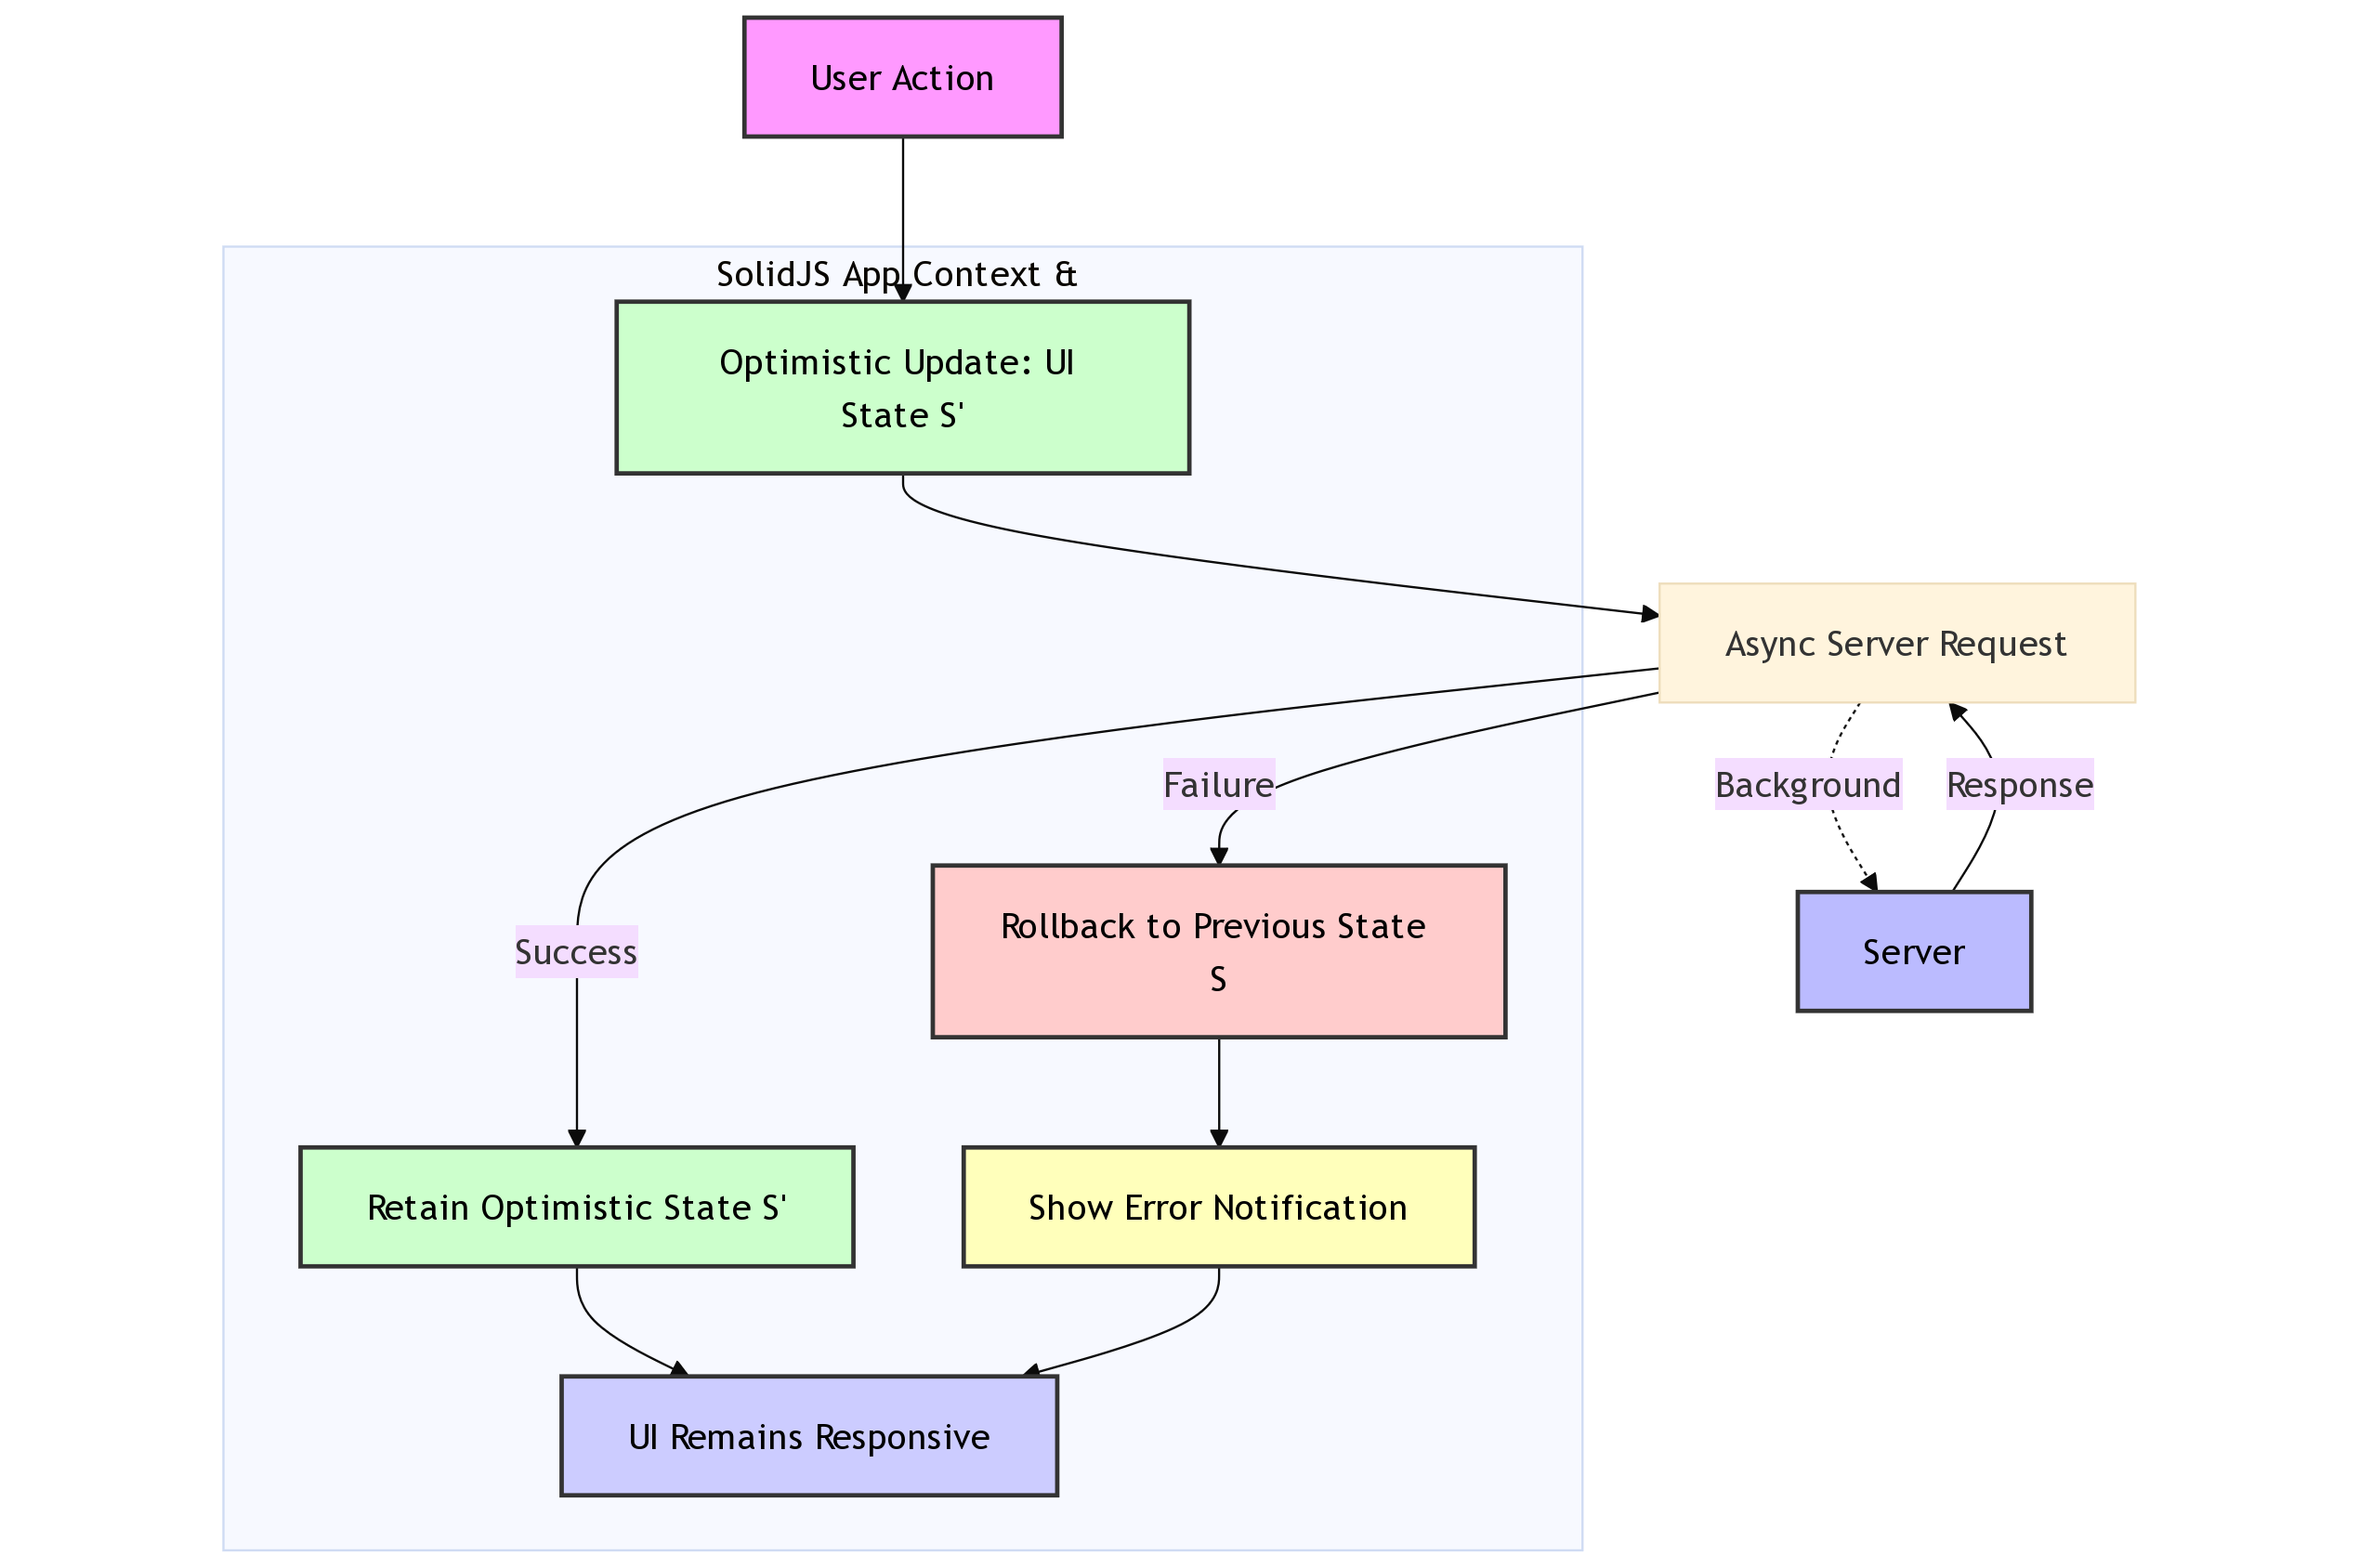
\includegraphics[width=0.85\textwidth]{opus_diagram.png}
\caption{OPUS System Architecture and Data Flow}
\label{fig:opus_architecture}
\end{figure}

\section{Current Optimistic Update Implementations in YipYap}
\subsection{Gallery File Uploads}
After upload, new items are added to the gallery UI before server confirmation. If the server fails, the UI is reverted and an error is shown.

\subsection{Caption Editing}
Caption changes are reflected in the UI immediately, with rollback on error.

\subsection{Favorites}
Favorite state is toggled in the UI before server confirmation, providing instant feedback.

\subsection{Tag Management}
Tag add, edit, and remove operations are performed optimistically, updating the UI instantly.

\subsection{Bounding Box Editing}
Add, update, and delete operations for bounding boxes are performed optimistically, ensuring a smooth annotation experience.

\section{Opportunities for Further Optimistic Updates}
\subsection{Git Operations}
Currently, the UI waits for server response before updating git status, branches, and related state. OPUS proposes optimistically updating git state in the UI, with rollback on error.

\subsection{Batch Operations}
Batch deletes and multi-item operations may not update the UI until server confirmation. OPUS recommends removing items from the UI immediately, with rollback if the server fails.

\subsection{Settings and Preferences}
Some settings changes are only reflected after server confirmation. OPUS suggests updating UI state immediately, with rollback on error.

\subsection{Gallery Deletion}
Deletion of images and folders may not be optimistic. OPUS proposes removing items from the UI immediately, with rollback if the server fails.

\subsection{Candidate Files for OPUS Integration}
The following files are prime candidates for further OPUS integration:
\begin{itemize}
    \item \texttt{src/composables/useGitManager.ts}
    \item \texttt{src/contexts/gallery.ts}
    \item \texttt{src/contexts/selection.ts}
    \item \texttt{src/components/Gallery/Gallery.tsx}
    \item \texttt{src/components/Settings/MemorySettings.tsx}
\end{itemize}

\section{Best Practices for Optimistic Updates in SolidJS}
OPUS recommends keeping update functions pure, handling errors gracefully with rollback and user notification, leveraging fine-grained reactivity for efficient updates, batching updates to minimize reactivity cycles, and providing clear feedback through the notification system. Thorough testing is essential to ensure rollback logic is robust and covers all edge cases.

\section{Conclusion}
OPUS demonstrates that optimistic UI updates, when combined with SolidJS's fine-grained reactivity, can deliver a highly responsive user experience. By expanding optimistic update patterns to more areas of YipYap---such as git operations, batch actions, and settings---the platform can further enhance user satisfaction and perceived performance.

\section{References}
\begin{thebibliography}{99}
\bibitem{solidstartoptimistic} Optimistic UI With SolidStart. Available: \url{https://www.brenelz.com/posts/optimistic-ui-with-solid-start/}
\bibitem{logrocketoptimistic} Understanding optimistic UI and React’s useOptimistic Hook. Available: \url{https://blog.logrocket.com/understanding-optimistic-ui-react-useoptimistic-hook/}
\bibitem{optimus} OPTIMUS v2.1: Performance-Optimized Direct API Integration with Progressive Loading for Large-Scale Data Selection in SolidJS Applications. Reynard Project Documentation.
\bibitem{solidjsdocs} SolidJS Documentation. Available: \url{https://www.solidjs.com/docs}
\end{thebibliography}

\end{document} 